\documentclass{article}

%Aus dem LaTex Template der Universit�t Stuttgart
%------------------------------------------------
\usepackage[utf8]{inputenc}
\usepackage[T1]{fontenc}
\usepackage[sfdefault]{ClearSans} %% option 'sfdefault' activates Clear Sans as the default text font
\usepackage{cmap}
\usepackage[ngerman]{babel}
\usepackage{graphicx}
\usepackage[pdftex,hyperref,dvipsnames]{xcolor}
\usepackage{listings}
\usepackage[a4paper,lmargin={2cm},rmargin={2cm},tmargin={3.5cm},bmargin = {2.5cm},headheight = {4cm}]{geometry}
\usepackage{amsmath,amssymb,amstext,amsthm}
\usepackage[lined,algonl,boxed]{algorithm2e}
\usepackage{tikz}
\usepackage{hyperref}
\usepackage{url}
\usepackage[inline]{enumitem} % Erm�glicht �ndern der enum Item Zahlen
\usepackage[headsepline]{scrpage2} 
\usepackage{algorithmic} % F�r Pseudocode
\usepackage{ marvosym } % f�r Pfeil(e)
\usepackage{booktabs} % F�r die sch�neren Booktabs-Tabellen
\usepackage{tikz}
\usepackage{pdfpages}
\usepackage{blindtext}
\usepackage{scrextend}
\usepackage{pdfpages}
\usepackage{natbib} % Yannis hat das importiert; TODO: nachfragen, zu was das gut ist
\pagestyle{scrheadings} 
\usetikzlibrary{automata,positioning}

\begin{document}
	%%% Obligatorisches Deckblatt
	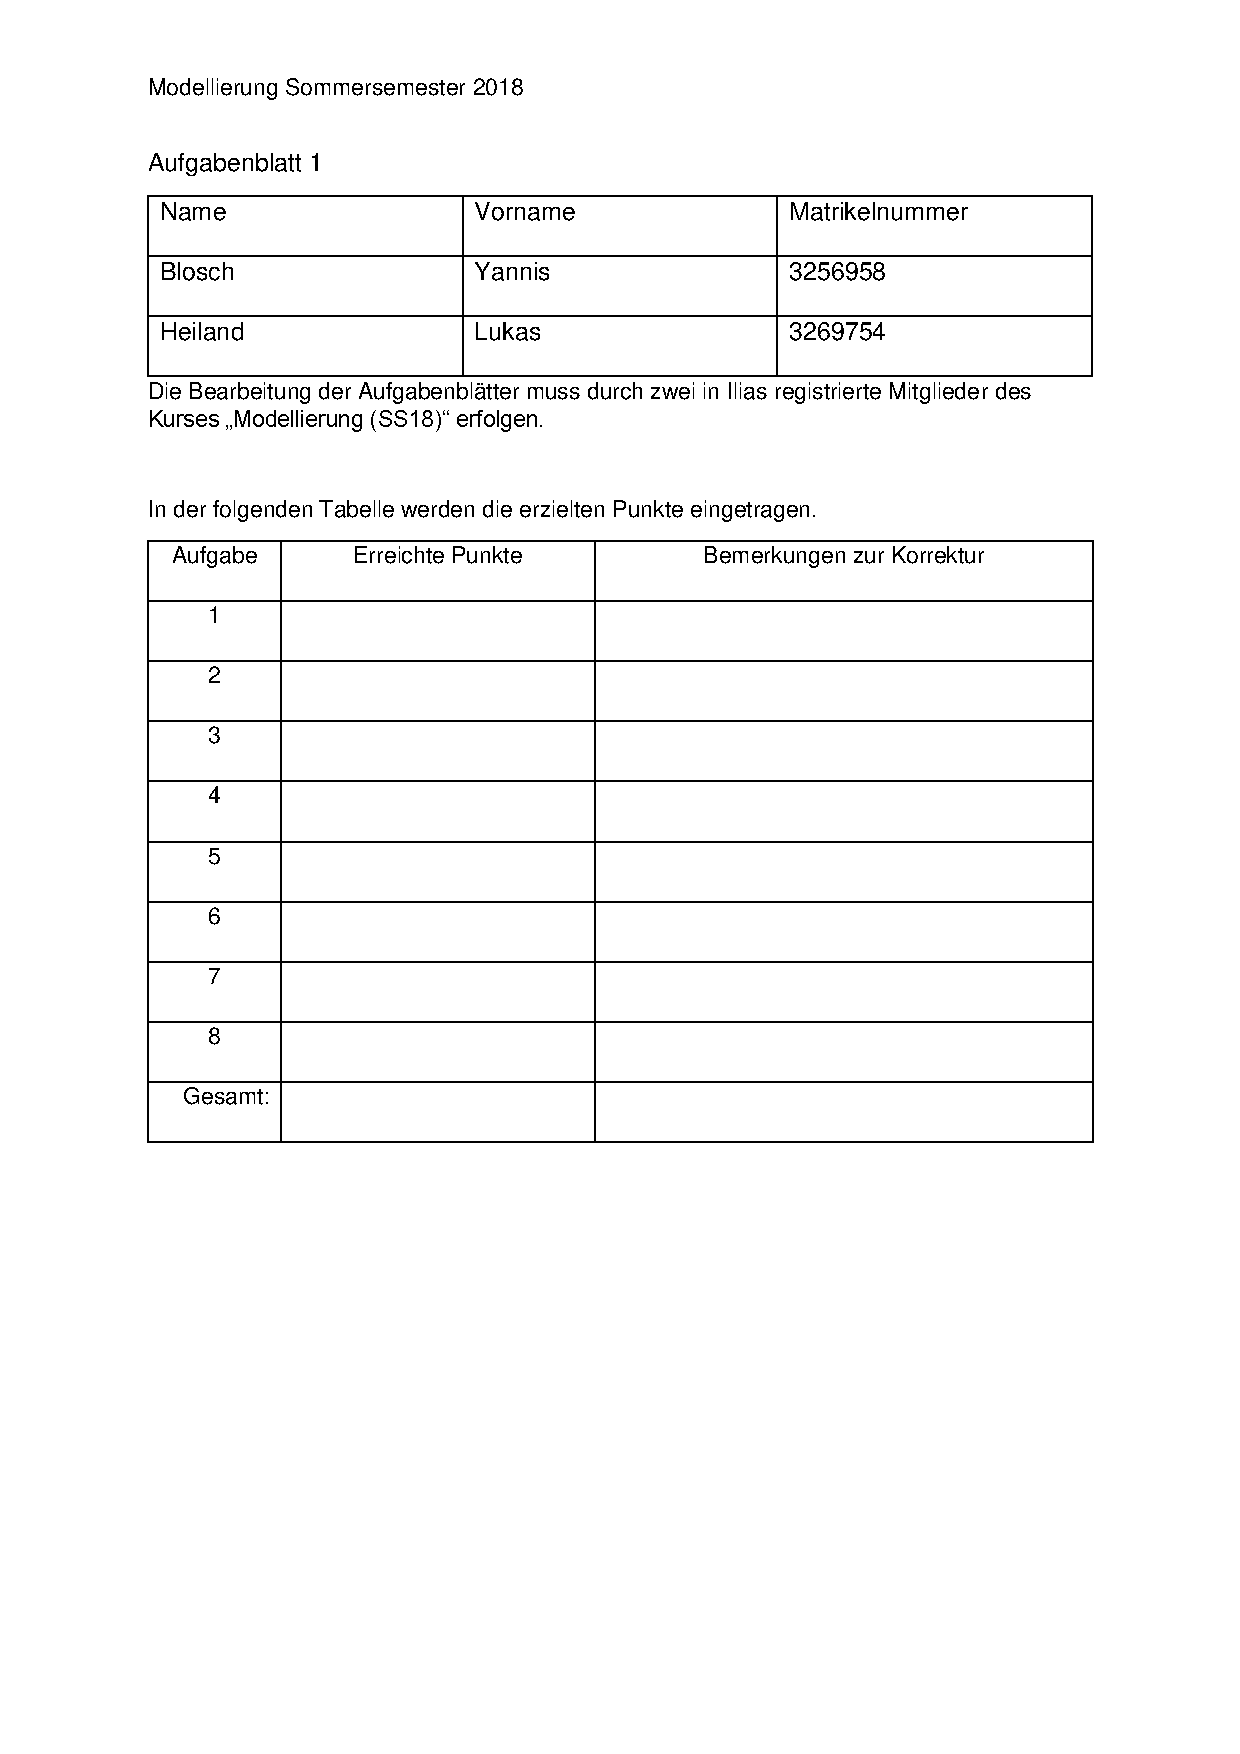
\includepdf[pages=-]{deckblatt.pdf}
	
	%%% Kopfzeile
	% Counter für das Blatt und die Aufgabennummer.
% Ersetze die Nummer des Übungsblattes und die Nummer der Aufgabe
% den Anforderungen entsprechend.
% Beachte:
% \setcounter{countername}{number}: Legt den Wert des Counters fest
% \stepcounter{countername}: Erhöht den Wert des Counters um 1.
\newcounter{sheetnr}
\setcounter{sheetnr}{1} % Nummer des Übungsblattes
\newcounter{exnum}
\setcounter{exnum}{1} % Nummer der Aufgabe

% Befehl für die Aufgabentitel
\newcommand{\exercise}[1]{\section*{Aufgabe \theexnum\stepcounter{exnum} #1}} % Befehl für Aufgabentitel

% Formatierung der Kopfzeile
% \ohead: Setzt rechten Teil der Kopfzeile mit
% Namen und Matrikelnummern aller Bearbeiter
\ohead{Yannis Blosch (3256958)\\
Lukas Heiland (3269754)}
% \chead{} kann mittleren Kopfzeilen Teil sezten
% \ihead: Setzt linken Teil der Kopfzeile mit
% Modulnamen, Semester und Übungsblattnummer
\ihead{Modellierung\\
Sommersemester 2018\\
Blatt \thesheetnr}
	
	
	
	%%% XML Schema instanziieren
	\section*{Aufgabe 11.1}
	<?xml version=\textquoteleft1.0\textquoteright encoding=\textquoteright UTF-8\textquoteright?>\\
	<Adresse>\\
	   \hspace*{10mm}<Name>Fakultät für Informatik der Universität Stuttgart</Name>\\
	   \hspace*{10mm}<Straße>Universitätsstraße 38</Straße>\\
	   \hspace*{10mm}<Stadt>Stuttgart</Stadt>\\
	   \hspace*{10mm}<Postleitzahl>70569</Postleitzahl>\\
	   \hspace*{10mm}<Land>DE</Land>\\
	</Adresse>
	
	
	
	%%% UML Zustandsdiagramm
	\section*{Aufgabe 11.2}
	
	
	
	
	%%% Petri-Netze
	\section*{Aufgabe 11.3}
	
	
	
	%%% Modellierung mit BPMN 2.0
	\section*{Aufgabe 11.4}
		\begin{figure}[h!]
			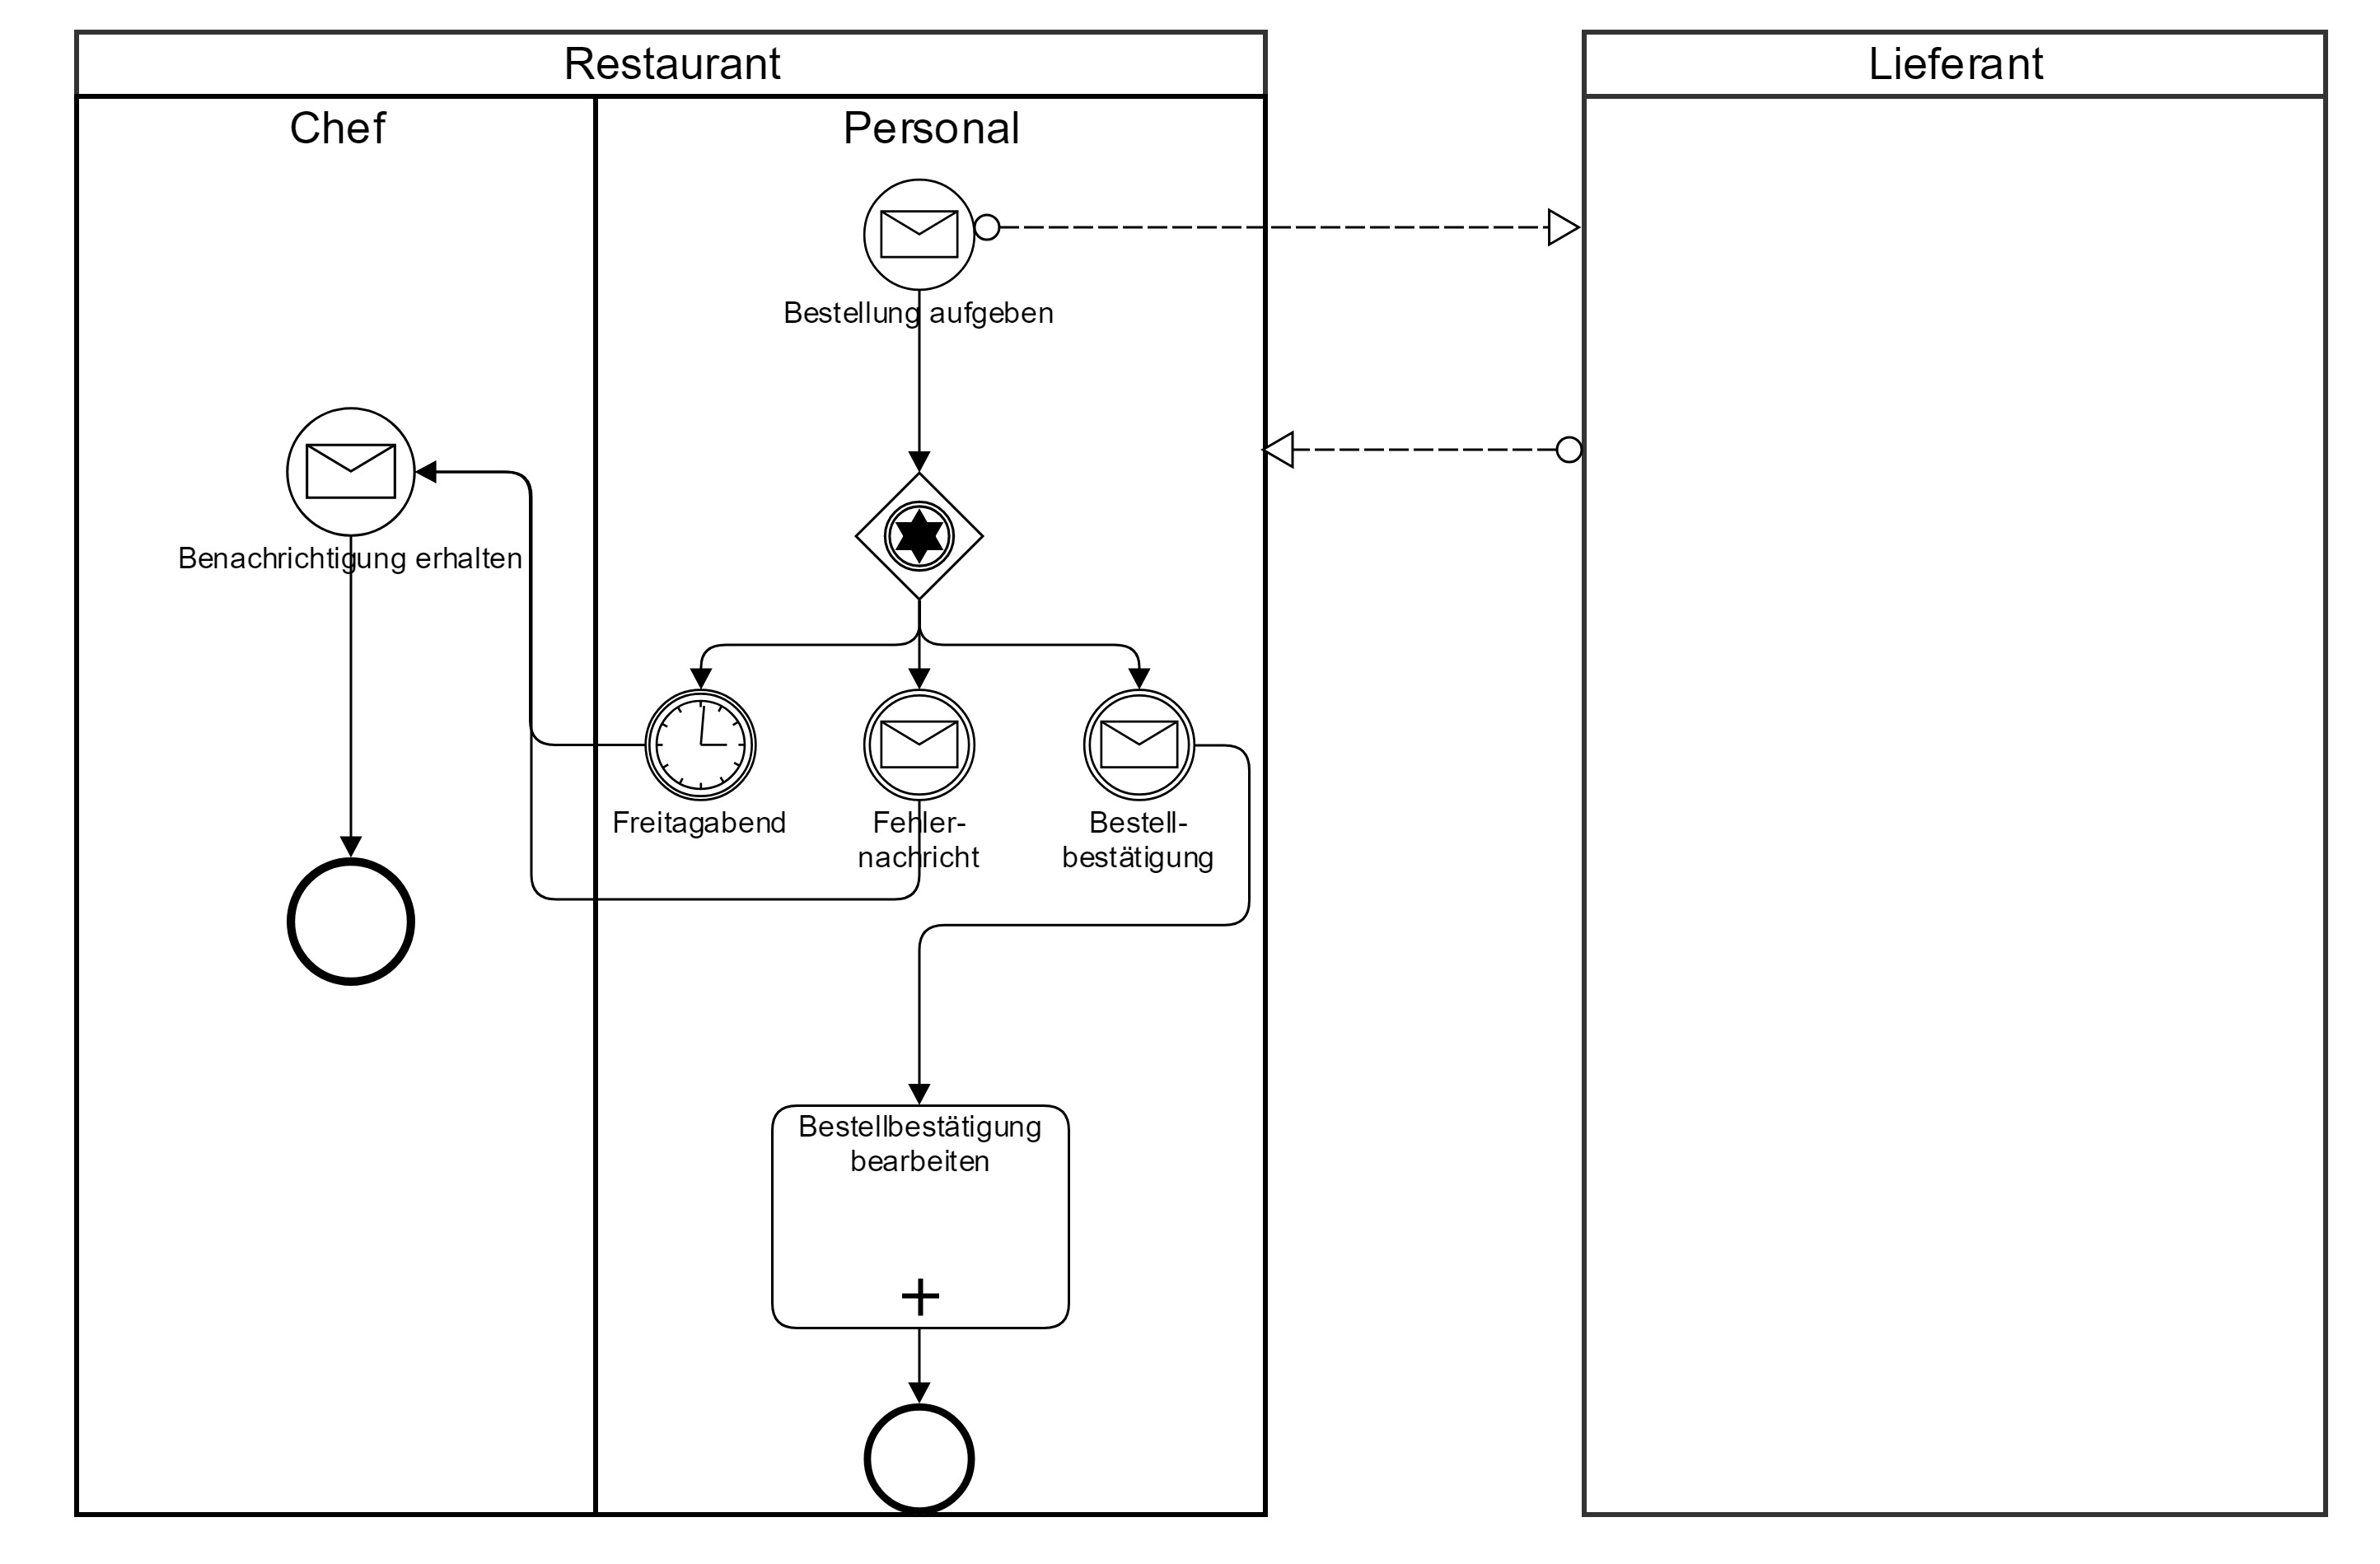
\includegraphics[scale=0.19]{aufgabe_11_4.jpg}
		\end{figure}
	\pagebreak
	
	%%% BPMN 2.0 Notation
	\section*{Aufgabe 11.5}
		\paragraph*{A:}Message Task
		
		\paragraph*{B:}Manual Task
		
		\paragraph*{C:}
		
		\paragraph*{D:}Service Task
		
		\paragraph*{E:}User Task
		
		\paragraph*{F:}Script Task
	
	
\end{document}